\chapter{Introduction}
\label{chap:introduction}

Transport Layer Security (TLS) is a cryptographic protocol that provides secure transport connection between applications over a computer network, e.g. web server and web browser. TLS is also referred to as Secure Socket Layer (SSL), its predecessor. Using TLS prevents eavesdropping, tampering and message forgery. It provides privacy and data integrity between communicating applications. The protocol secures transmitted data using encryption. It offers server and, optionally, client authentication to confirm the identities of parties involved in the communication. The integrity check value implemented in the protocol provides integrity of the transfered data. \cite{RFC5246}

\section{Structure of the TLS protocol}
\label{sec:stucture}

The TLS security protocol is layered between the application protocol layer and TCP/IP layer according to the Internet Model (or between Session and Transport layers according to the OSI Model), where it can secure and then send application data to the transport layer \cite{ms:overview}. Thus it can support multiple application layer protocols, such that HTTP, FTP, SMTP, POP3 and other. The protocols using TLS become respectively HTTPS, FTPS, SMTPS, POP3S and so on.

The TLS protocol can be splited into two layers. The lowest layer of the TLS is the Record Protocol. The upper layer is the Handshake layer, that consists of the following protocols: Handshake Protocol, ChangeCipherSpec Protocol, Alert Protocol. Figure \ref{fig:tls_structure} illustrates the srtucture of the TLS protocol. 


\begin{figure}[H]
	\centering
		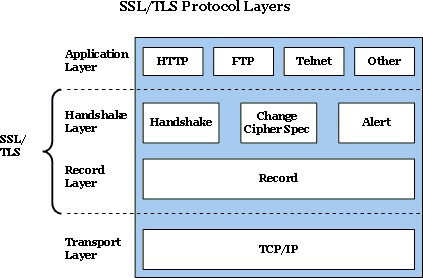
\includegraphics[scale=0.85]{images/tls_structure.jpg}
	\caption{TLS Protocols Structure \cite{ms:overview}}
	\label{fig:tls_structure}
\end{figure}

\section{Record Protocol}
\label{sec:record_protocol}

The connection with two independent channels is established through the TLS Handshake, from the client to the server and in the other direction from the server to the client. The Record Protocol is responsible for the data protection on these channels using the authenticated encryption scheme. The processing of data 
Firstly the Record Protocol layer receives the data from the application layer. Then it fragments the data to a size appropriate to the cryptographic algorithm. compress or decompress 


\section{Benefits/Drawbacks, Properties, Characteristic}
\label{sec:introduction_suggestions}

% \begin{itemize}
%	\item Create a BFH Style Files
%	\item Template for the Compilation of presentations with \LaTeX{}
% \end{itemize}


